\chapter{Background and Literature Review}\label{C:ex}
\section{Background}
\subsection{\emph{QoS}-Aware Web Service Composition}

Web services \cite{24} are modular, distributed, self-contained, dynamic applications that are published on the Web in order to be available to users. They follow certain technical standards such as Simple Object Access Protocol (SOAP) \cite{24} for accessing Web services, Web Service Description Language (WSDL) \cite{24} for describing Web services, and Universal Description, Discovery and integration (UDDI) \cite{25} for describing, publishing, and finding web services. \par

Web Services are an important component of the internet, since they can be $'$called$'$ by software and thereby provide functionality found on other sites. In essence, a web service is any piece of software that makes itself available over the internet \cite{27}.\par

For example, if I post pictures on Flicker about various steps needed to build my house, I may wish to dynamically display certain pictures. However, the relevant images are not stored on my local storage, but on Flicker. In this case I can make a dynamic request to ask Flicker to provide me with an image, since Flicker provides such a Web service.\par

However, it is important to note that a single Web service may only provide limited functionality, which is not sufficient to respond to the user's request. In order to complete complex tasks, a range of Web services are required, and it is necessary to combine, or compose these Web services to provide new value-added and complex functionality \cite{28}. When a user's request cannot be fulfilled by any available web service then Web Service Composition is required to fulfill the user's request.\

Web service composition is the process of combining several Web services into a more complicated and powerful service. Since there is no uniform definition, different researchers have defined the Web service composition problem from different perspectives \cite{22,21,23,20}. In \cite{20}, from the point of view of business processes, Web service composition is regarded as the organic connection of services according to certain business rules, so that companies can cooperate with each other to reach certain established business goals. In \cite{21}, from the perspective of application integration, Web service composition is the process of seamlessly integrating heterogeneous information systems and software from different enterprises, eliminating information silos and forming interconnected software consortia. In \cite{22}, from the point of view of problem solving, Web service composition is considered to be a way to achieve user-specific objectives, and a combination service satisfying this goal is found in a given set of services. In \cite{23}, from the point of view of task planning, service composition is a process of decomposing a large task into several subtasks, and breaking down these subtasks into even more smaller subtasks.\par

This project considers Web service composition to be the process of synthesizing several Web services when a single Web service can not meet a user's requirements, so as to form a large-scale composite service with internal process logic.\par

Nowadays, a large number of Web services on the Internet provide the same or overlapping functionality but present different non-functional characteristics. These non-functional characteristics are called quality of service (\emph{QoS}) properties, such as response time, execution cost, availability, reliability etc. Each of those properties are described in detail in the next section. Because \emph{QoS} properties have became the most commonly used set of characteristics for measuring the quality of Web services, meeting global \emph{QoS} requirements while fulfilling various functional requirements is called the problem of \emph{\emph{QoS}-aware Web service composition} \cite{26,28}.


\subsection{\emph{QoS} Properties}
Quality of service (\emph{QoS}) is one of the important factors to consider when composing services. It defines the non-functional requirements of a service, such as response time, execution cost, availability, reliability etc. Good quality of service means achieving certain \emph{QoS} goals which are termed \emph{QoS} values or \emph{QoS} properties. These \emph{QoS} properties indicate whether a Web service is reliable, trustworthy or efficiency. Their significance stems from the fact that a Web service may be functionally capable of performing a given task, but might not be reliable or efficient enough to achieve users' satisfaction. Web services are usually rated using multiple \emph{QoS} values, each value representing an aspect, or \emph{QoS} property, of the Web service. \emph{QoS} properties are the most commonly used characteristics for measuring the quality of Web services and even composite services, as they indicate whether a service is capable of meeting users' expectations.\par

To model the performance of service compositions we considered four \emph{QoS} attributes: \emph{availability, reliability, execution cost} and \emph{response time}. We chose these because they are commonly used in this field \cite{15,14,16,4}. According to \cite{11,4,18}, the four above-mentioned \emph{QoS} properties are defined as follows:\par

\emph{Execution Cost} is the amount of money that a service requester has to pay for using the Web service. The global \emph{execution cost} \emph{$C_t$} of a composite set of services can be treated as the sum of the execution costs of all the operations invoked by the services \emph{s} used. 

$$C_t = \sum_{i=1}^{|s|} C_i$$

\begin{example}[Example: \emph{Execution Cost}]
\noindent
The total \emph{execution cost} of the composite service in Figure 2.1 is total execution \emph{$C_t$}:
\begin{equation}
 C_t = Cost(S_1) + Cost(S_2) + Cost(S_3) + Cost(S_4)
 \end{equation}

\end{example}
\setlength{\textfloatsep}{20pt}% Remove \textfloatsep

The \emph{response time} of a single task is the time which elapses between sending a task request and receiving a response. Web service composition allows services to execute in parallel. Thus, when considering a step where two tasks execute in parallel, the path with the longest \emph{response time} is chosen to calculate the time taken for that step.\par
\begin{example}[Example: \emph{Response Time}]
\noindent
In Figure 2.1, which shows an example Web service composition, services $S_{2}$ and $S_{3}$ can be executed in parallel. The \emph{response time} depends on $S_{2}$ and $S_{3}$'s local \emph{QoS} duration property values. If $S_{2}$'s \emph{QoS} duration property value is greater than $S_{3}$'s \emph{QoS} duration property value, then the overall \emph{response time} of the composite service can be computed as the sum of all three service nodes $S_{1}$, $S_{2}$ and $S_{4}$'s local \emph{QoS} duration property values.\par
\end{example}
\setlength{\textfloatsep}{20pt}% Remove \textfloatsep

\emph{Availability} is defined as the ratio of (1) the time during which a service is ready for use and (2) the time during which the Web service exists. The global availability \emph{$A_t$} of a composite Web services can be computed as the product of the local availabilities of the Web services \emph{s} used in the service composition.
 $$A_t = \prod_{i=1}^{|s|} A_i$$

\begin{example}[Example: \emph{Availability}]
\noindent
The \emph{availability} of the composite service in Figure 2.1, can be computed as:
\begin{equation}
 A_t = Availability(S_{1}) \times Availability(S_{3}) \times  Availability(S_{2}) \times Availability(S_{4}) 
  \end{equation}
\end{example} 
\setlength{\textfloatsep}{20pt}% Remove \textfloatsep


\emph{Reliability} is the how reliable message delivery is to the Web service within the maximum permitted time frame. Global \emph{reliability} \emph{$R_t$} can be calculated as the product of the local reliabilities of the Web services \emph{s} used in the service composition.
 $$R_t = \prod_{i=1}^{|s|} R_i$$
\begin{example}[Example: \emph{Reliability}]
\noindent
 The \emph{reliability} of the composite service in Figure 2.1, 
can be computed as:
 \begin{equation}
  R_t = Reliability(S_{1}) \times Reliability(S_{3}) \times Reliability(S_{2}) \times Reliability(S_{4})
    \end{equation}

 \end{example}
\setlength{\textfloatsep}{20pt}% Remove \textfloatsep

\begin{figure}[H]
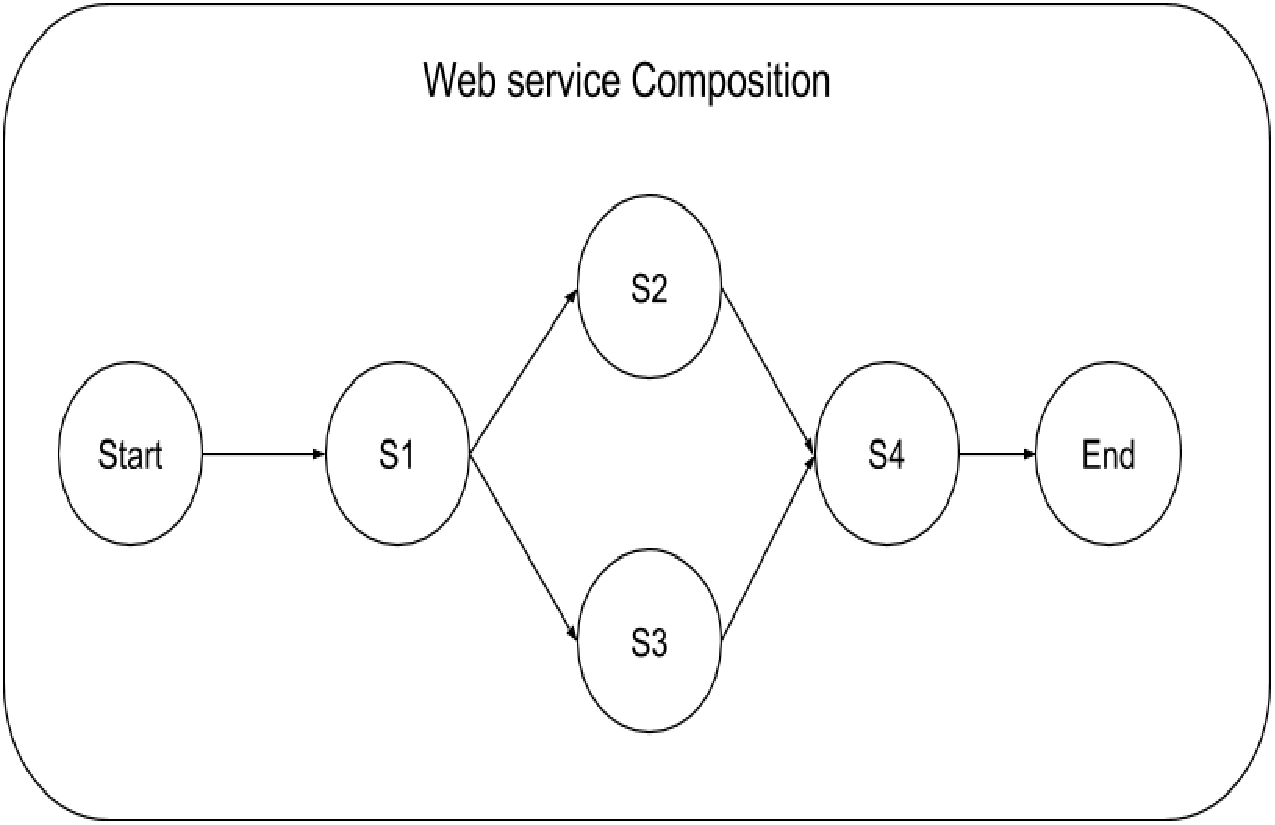
\includegraphics[width=9cm]{Figure2-1ExampleWebServiceComposition.pdf}
\centering
\caption{Example Web service composition}
\end{figure} 

\subsection {\emph{QoS}-Aware Fitness Functions} \label{fitnessFunction}

To evaluate the quality of a Web service composition we need a suitable fitness function. A fitness value can be used to reflect the global quality of service of a service composition. Following the common practice  \cite{19,14,4} used in multi-criteria optimization problems, we normalize the values of each \emph{QoS} property and restrict them to the interval [0,1]. We choose the same objective function as that we used in \cite{19,4} for our approach. The fitness for candidate \emph{i} is defined as follows:
\begin{equation}
Objective_{i}=(w_{1} \times A_{i}) + (w_{2} \times R_{i}) + (w_{3} \times T_{i}) + (w_{4} \times C_{i})
\end{equation}
\noindent
where \emph{A$_{i}$}, \emph{R$_{i}$}, \emph{T$_{i}$} and  \emph{C$_{i}$} denote the normalized availability, reliability,  execution cost and  execution time of candidate \emph{i}, and weights \emph{w} are real positive numbers where $w_{1} + w_{2} + w_{3} + w_{4} = 1$. The value of weights assigned by the user to the objective function represents the importance of the different \emph{QoS} properties for the Web service composition. \par

To achieve normalization we take the minimum and maximum values of all the composition solutions discovered so far. We then use those values to normalize the \emph{QoS} properties according to the following formula \cite{4}:


\[A_i = \left\{
\begin{array}{l l} 
    \frac{A_i - A_{min}}{A_{max} - A_{min}}      & \quad \text{if  } A_{max} - A_{min} \neq 0\\
    1  & \quad \text{if  } A_{max} - A_{min} = 0\\
\end{array} \right. \]\label{eq:2}
\[R_i = \left\{
\begin{array}{l l} 
    \frac{R_i - R_{min}}{R_{max} - R_{min}}      & \quad \text{if  } R_{max} - R_{min} \neq 0\\
    1  & \quad \text{if  } R_{max} - R_{min} = 0\\
\end{array} \right. \]\label{eq:2}
\[T_i = \left\{
\begin{array}{l l} 
    \frac{T_{max} - T_i}{T_{max} - T_{min}}      & \quad \text{if  } T_{max} - T_{min} \neq 0\\
    1  & \quad \text{if  } T_{max} - T_{min} = 0\\
\end{array} \right. \]\label{eq:2}
\[C_i = \left\{
\begin{array}{l l} 
    \frac{C_{max} - C_i}{C_{max} - C_{min}}      & \quad \text{if  } C_{max} - C_{min} \neq 0\\
    1  & \quad \text{if  } C_{max} - C_{min} = 0\\
\end{array} \right. \]\label{eq:2}

Normalized \emph{QoS} property values close to \emph{1} indicate better quality, while normalized values closer to \emph{0} indicate poorer quality. Finally, we use the normalized \emph{QoS} properties and weights to calculate the fitness of the individual candidates, where the largest fitness value will be chose as the best Web service composition out of that set of candidates. 

\subsection{Neo4j Graph Database}
A graph database is a type of \emph{NoSQL} database, which uses graph theory to store, map and query relationships. Graph databases contains \emph{nodes} and \emph{edges} components \cite{30}. They are widely used to model social networks and also used to solve real-world problems. \emph{Transportation} \cite{32}, \emph{protein-interaction} \cite{33} and even \emph{business networks} \cite{34} can naturally be modeled as graphs. Paper \cite{30} evaluates four current types of graph databases (\emph{Neo4j} \cite{6}, \emph{OrientDB} \cite{35}, \emph{Titan} \cite{36} and \emph{DEX} \cite{37})  from a performance point of view. The results show that the \emph{Neo4j} graph database gets the best performance with \emph{loading datasets}, \emph{finding the shortest path} and \emph{breadth-first exploration of nodes neighbourhood}. Good traversal performance reduces the time taken for Web service composition. \par

Because of it's good performance, we employed a \emph{Neo4j} \cite{6} graph database for our project. We also chose it because it is suitable for representing connected and directed Web services and it allows for very fast retrieval, traversal and navigation of data. Our project used a \emph{Neo4j} graph database to store all services as \emph{nodes} and dependencies between the services as \emph{relationships} (edges). We gave all \emph{nodes} and \emph{relationships} their own individual properties. And for each data set we needed to create a graph database only once, after which we were able to use the database to solve various composition problems. \par

\section{Literature Review}
Over the past few years, Web services have become widely used. A large number of complex applications can be developed using compositions of existing services. Automatic Web service composition technology has become a major focus and challenge in building robust applications which make use of distributed services which provide various functions \cite{29}. Many approaches have been developed for Web service composition     4682364384283    which graph based approach shows its promise in generating feasible composition solutions efficiently, but only a few of them use the concept of graph theory. In this section, we will present a brief overview of some graph-based techniques that deal with automatic Web service composition.
\par

Da Silva et al. presents in \cite{2} an evolutionary computation technique that performs fully automated Web service composition using graph representations for solutions. There are two steps. The first step is to initialise the population by employing a graph building algorithm based on the planning graph approach described in composition literature \cite{3}. The second step is to perform mutation and crossover operations on selected candidates, to generate a new set of candidates and evaluate the fitness of those candidates.\par
The drawback of the approach in \cite{2} is that the graph mutation space contains many invalid service compositions that either violate the constraints of service dependencies or deteriorate the overall performance. Another disadvantage is that the system saves all the Web service dependencies in memory. With every new service request, this approach needs to regenerate all the dependencies again which incurs expensive computation costs. Furthermore, the cost of executing the graph building algorithm is high, since the graph building algorithm is employed twice, in two different processes, namely in the process of generating initial populations and the process of performing mutation and crossover operations.\par
Seyyed et al. \cite{5} uses a graph search algorithm to construct Web service compositions. This algorithm is based on input-output dependencies of Web services. In order to solve the service composition problem, the authors divide the process into two steps. The first step is to look for Web services which can potentially participate in the composition, and the second step is to find a corresponding composition. The graph building algorithm constructs edges between directly related Web services which have data dependencies between the inputs and outputs of these services. The main shortcoming of this approach is that semantic functions are not considered in the dependencies between input and output parameters. Thus there is no guarantee that a generated composite service will provide the precise functionality requested by the user.\par
The Web service composition approaches proposed by Da Silva et al. in \cite{2} and Seyyed et al. in \cite{5}, also share a common drawback. They do not include quality of service in their approach. This means the resulting Web services may not perform tasks that meet a user's non-functional requirements.\par

Jing et al \cite{26} developed a relational-database approach to constructing Web service compositions. This approach overcomes a major limitation of most automated service composition methods \cite{2,5}, which was to store Web services and dependencies between them only in memory. \cite{26} stored Web services and dependencies between the Web services in a database instead of memory. The authors propose an algorithms that builds a path between services in the service repository. According to their method, each path has a PathID, and input and output values. After all paths have been generated, they are then stored in the database. To handle the task request, a query must be sent to the database to find Web service composition paths which satisfy the request. The next step involves ranking and filtering the paths returned from the algorithms according to their \emph{QoS} value. The top rank will be the best composition for a given task. \par
One of the major drawbacks of the approach in \cite{26} is that it cannot efficiently handle a very large service repository. The proposed method is slow, as it preprocesses all the Web services in advance to generate paths between services which it stores in the database. However, if any service inputs or outputs have changed or any new Web services have been added, this will affect most of the paths stored in the database, since they are interconnected each other. In addition, many services offer identical or overlapping functionalities.\par
The result is that the number the paths in the database is enormous. And all the paths need to be processed in order to find the PathID and process the input and output of the each path in the related paths. So when creating web service compositions this greatly downgrades overall performance. The third drawback of the approach in \cite{26} is that it only considers the response time property when dealing with \emph{QoS}-aware Web service composition and does not consider execution cost, availability and reliability of the composition. This means the solution may not be the optimised solution.\par


As we have seen above, existing graph-based \cite{5} and GP based \cite{2} approaches need to build a data dependency graph for each given task. However, database dependencies between services in a service repository remain stable for all service tasks. Therefore, once a service dependency graph is generated it is best stored so it can be  used for all service tasks. In this project, we propose to use a graph database to store the information related to services and dependencies of services of a service repository. Once a graph database has been created using information in the service repository, all the services and dependencies of the services are permanently stored on local storage, and a Graph database like Neo4j, which has built-in path-finding methods is used. Unlike the relational-database approach in \cite{26},  in which there is a need to generate all the paths between services and then store those paths in the database. With each new service task, our approach can utilise existing dependency information contained within graph database dependency graphs. Our approach also takes the quality of service (\emph{QoS}) into consideration by including \emph{QoS} properties with each edge between Web services.\par   
 
In summary, most current non-database-type automated Web service composition methods \cite{2,5} are in-memory methods, which lead to Web service composition results, details of services and dependencies between services being stored, on local storage in simple text format. This means the reusability of the solution is very low, as much information is not stored, especially in the case of service dependencies and services are not reusable after memory is cleared. The relational-database-based approach \cite{26} uses stored services with dependencies between services stored in the database as paths. But the performance of SQL queries on the large resulting database as well as database maintenance is very low.\par